\documentclass{standalone}
\usepackage{pgfplots}
\pgfplotsset{compat=1.13}
\usepackage{amsmath}

\begin{document}

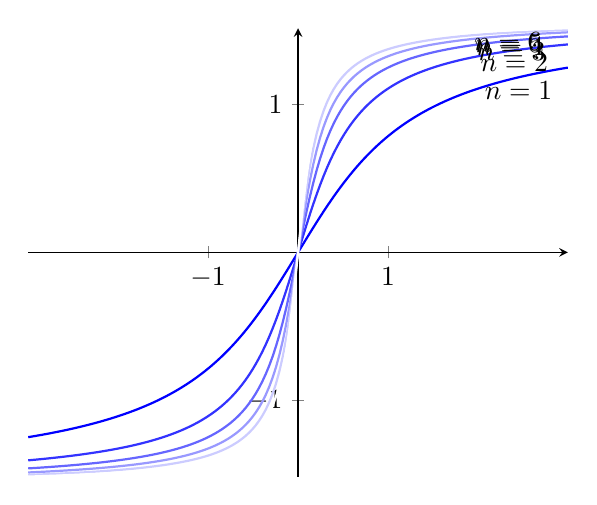
\begin{tikzpicture}
    \begin{axis}[
            axis y line = center,
            axis x line = center,
            xtick       = {-1,0,1},
            xticklabels = {$-1$,$0$,$1$},
            % ytick       = {-1,0,1},
            % yticklabels = {$-1$,$0$,$1$},
            samples     = 160,
            domain      = -3:3,
            xmin = -3, xmax = 3,
            % ymin = 0, ymax = 1,
        ]
        \foreach[evaluate=\n as \redfrac using (\n-1)*100/(6-1)] \n in {1,...,6}{
                \edef\temp{
                    \noexpand\addplot[white!\redfrac!blue, thick, mark=none, text = black] {atan(x*\n)*pi/180} node[pos=0.9, below right] (mid) {};
                    \noexpand\node[black] at (mid) {$n =\n$};
                }
                \temp
            }
    \end{axis}
\end{tikzpicture}

\end{document}